\documentclass[10pt]{article}

\usepackage{amsfonts,amssymb}
\usepackage[utf8]{inputenc}
\usepackage[english,russian]{babel}
\usepackage{graphicx}
\usepackage{mathtools}
\usepackage{multicol}
\usepackage{ textcomp }
\usepackage[colorlinks,urlcolor=blue]{hyperref}

\newcommand{\argmin}{\mathop{\rm arg\,min}\limits}
\newcommand{\argmax}{\mathop{\rm arg\,max}\limits}
\newcommand{\sign}{\mathop{\rm sign}\limits}
\newcommand{\cond}{\mspace{3mu}{|}\mspace{3mu}}
\def\RR{\mathbb{R}}
\def\XX{\mathbb{X}}
\def\EE{\mathbb{E}}
\def\NN{\mathcal{N}}
\def\LL{\mathcal{L}}
\def\YY{\mathbb{Y}}

\textheight=220mm
\textwidth=160mm

\title{Школа анализа данных\\ Восстановление зависимостей \\Домашнее задание №2}
\author{Кошман Дмитрий}
\date{}

\begin{document}
	
	
	\voffset=-20mm
	\hoffset=-17mm
	\font\Got=eufm10 scaled\magstep2 \font\Got=eufm10
	
	
	\maketitle
	
	\bigskip
	
	\textbf{Задача 1}
	
	\medskip
	
	На первом графике изображены приближения зависимости полиномами разных степеней. На втором - средняя квадратичная ошибка на наблюдаемых (train) и истинних (test) ответах, сэмплированных из интервала $[0, 2]$.
	
	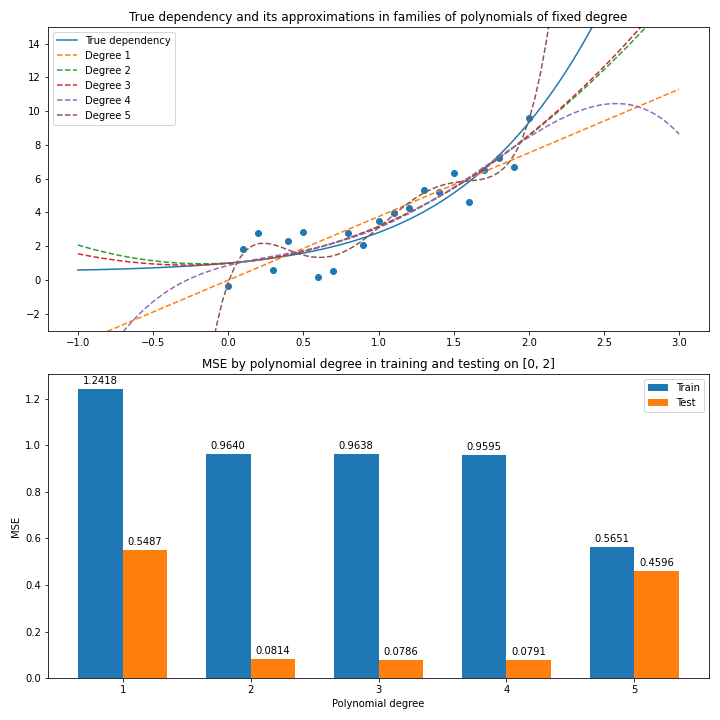
\includegraphics[width=.8\textwidth]{dependency hw2 task1.png}
	
	Как видно, полином 5 степени лучше приближает наблюдаемые данные, что ожидаемо, поскольку он из более широкого класса функций. Но истинную зависимость лучше всего приближают полиномы 2, 3 и 4 степени, тогда как полином 1 степени не улавливает закономерностей в данных, а 5 степени подстраивается под случайный шум.
		
	\bigskip
	
	\textbf{Задача 2}
	
	\medskip
	

	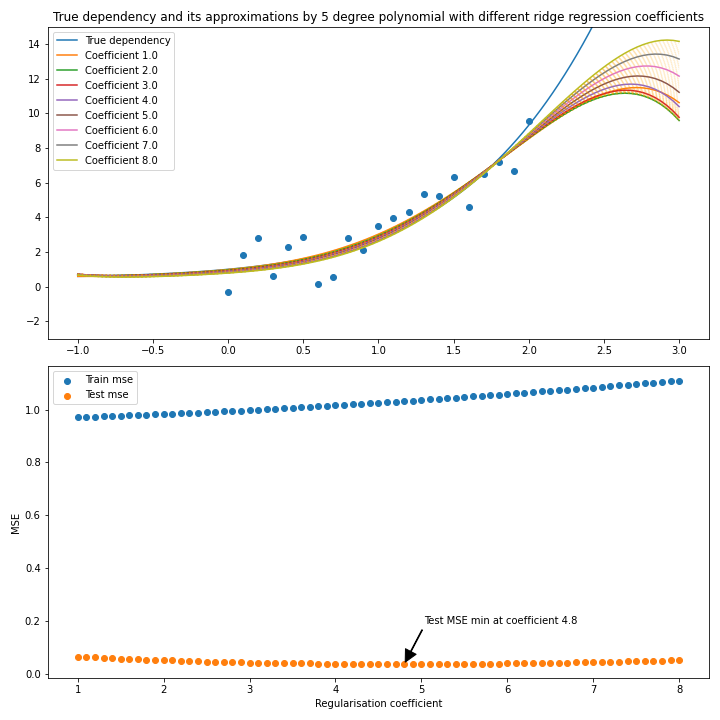
\includegraphics[width=.8\textwidth]{dependency hw2 task2.png}
	
	Наиболее точная оценка достигается при параметре регуляризации, равным $4.8$.
	
	\bigskip
	
	\textbf{Задача 3}
		
	\medskip
	
	Получим оценку параметра $\hat{\lambda }$ с помощью метода максимального правдоподобия:
	
	$$\hat{\lambda } = \argmax_\lambda \prod_{i=1}^{52} p_{n_i} = \argmax_\lambda \sum_{i=1}^{52} \ln \frac{\lambda^{n_i}}{n_i!}e^{-\lambda} = $$
	
	$$= \argmax_\lambda \sum_{i=1}^{52} (n_i \ln \lambda - \ln n_i! - \lambda) = \argmax_\lambda (- 52\lambda + \ln \lambda\sum_{i=1}^{52} n_i )  =$$
	
	$$ = \frac{\sum_{i=1}^{52} n_i}{52}$$
	
	\bigskip
	
	\textbf{Задача 4}
	
	\medskip
	
	Получим оценку параметров $\hat{a}, \hat{M}$ с помощью метода максимального правдоподобия:
	
	$$(\hat{ a }, \hat{M}) = \argmax_{a, M} \prod_{i=1}^{n} \frac{1}{a} [M-a/2 \leq x_i \leq M + a/2] = $$
	
	$$ = \argmax_{a, M}  \frac{1}{a^n} [M-a/2 \leq x_{(1)}; x_{(n)} \leq M + a/2] = $$
	
	$$ = \left( x_{(n)} - x_{(1)}, \frac{ x_{(n)} + x_{(1)} }  {2} \right)$$
	
	
\end{document}=

